\documentclass[11pt,a4paper]{article}

% --- Layout ---
\usepackage[margin=1in]{geometry}
\usepackage{microtype}
\usepackage{setspace}
\usepackage{titling}

% --- Math & symbols ---
\usepackage{amsmath, amssymb, amsthm}
\usepackage{mathtools}
\usepackage{bm}

% --- Graphics & tables ---
\usepackage{graphicx}
\usepackage{tikz}
\usetikzlibrary{arrows.meta, positioning, fit, calc}
\usepackage{booktabs}
\usepackage{multirow}
\usepackage{array}
\usepackage{xcolor}
\usepackage{subcaption}

% --- Algorithms ---
\usepackage{algorithm}
\usepackage{algpseudocode}

% --- Citations ---
\usepackage[numbers,sort&compress]{natbib}
\usepackage{hyperref}
\usepackage{url}
\hypersetup{
    colorlinks=true,
    linkcolor=blue!50!black,
    citecolor=green!50!black,
    urlcolor=red!50!black,
}

% --- Code listings ---
\usepackage{listings}
\lstset{
    basicstyle=\ttfamily\small,
    breaklines=true,
    frame=single,
    showstringspaces=false,
}

% --- Theorem environments ---
\newtheorem{theorem}{Theorem}
\newtheorem{proposition}[theorem]{Proposition}
\newtheorem{lemma}[theorem]{Lemma}
\newtheorem{corollary}[theorem]{Corollary}
\theoremstyle{definition}
\newtheorem{definition}[theorem]{Definition}
\newtheorem{assumption}[theorem]{Assumption}
\theoremstyle{remark}
\newtheorem{remark}[theorem]{Remark}

% --- Custom macros ---
\newcommand{\budget}{\mathcal{B}}                 % token compute budget
\newcommand{\Acc}{\mathrm{Acc}}                    % accuracy
\newcommand{\policy}{\pi}                           % policy LLM
\newcommand{\polacc}{\alpha(\policy)}              % per-level (pillar) accuracy of policy
\newcommand{\gain}{\Delta}                          % marginal search gain
\newcommand{\mctstax}{\textsc{MCTS-Tax}}           % MCTS over CWE taxonomy
\newcommand{\mctsreas}{\textsc{MCTS-Reason}}       % MCTS over reasoning trajectory
\newcommand{\TODO}[1]{\textcolor{red}{\textbf{[TODO: #1]}}}

% --- Title ---
\title{When Does Test-Time Search Help LLMs Classify Vulnerabilities?\\
A Compute-Matched Study of MCTS over Taxonomy and Reasoning}

\author{%
  Anonymous Authors%
  % Replace with real authors after de-anonymization phase.
}

\date{}

\begin{document}
\maketitle

\begin{abstract}
% Pitch (1-2 sentences): the problem and why it matters.
Test-time search --- self-consistency, best-of-$N$, beam search, and Monte Carlo
Tree Search (MCTS) --- is increasingly applied to make large language models (LLMs)
reason more reliably. Yet reported gains often compare a search method running
many model calls against a single greedy call, conflating the value of \emph{search}
with the value of \emph{extra compute}.
%
% Gap (1 sentence): what's missing.
It remains unclear not only \emph{when} structured search helps an LLM, but
\emph{what it should search over}.
%
% Contribution (2-3 sentences): what we do.
We present a controlled, \textbf{compute-matched} study of test-time search for
hierarchical vulnerability classification over the Common Weakness Enumeration
(CWE) taxonomy. Holding the policy LLM, prompt, and token budget fixed, we compare
search strategies and isolate three axes the literature entangles: \emph{policy
strength}, \emph{reward fidelity} (self-evaluation vs.\ a stronger external judge),
and---most consequentially---the \emph{search space}, contrasting MCTS over the
output taxonomy against MCTS over a free-form reasoning trajectory.
%
% Results: the numbers.
Three findings on a code-vulnerability benchmark (BigVul, patch-diff inputs).
(i) \emph{What you search over dominates}: MCTS over a reasoning trajectory beats
MCTS over the taxonomy by $+12$ leaf-accuracy points at \emph{half} the token
budget ($p{<}10^{-4}$), because taxonomy search commits to a wrong coarse
category on $60\%$ of examples and cannot recover, whereas reasoning search
defers commitment; moreover its accuracy is flat in the iteration knob, so the
gain comes from the reasoning \emph{scaffold} rather than the search machinery.
(ii) Search compensates \emph{weak} policies (up to $+8$ points over greedy) but
not strong ones, and its gain shrinks monotonically with policy strength;
self-consistency (sampling without a reward) captures almost none of it.
(iii) A stronger external judge leaves taxonomy search unchanged and does not
survive budget matching on reasoning search---the bottleneck is the policy and
the search space, not reward fidelity.
%
% Impact (1 sentence): why this matters beyond the paper.
We conclude that the design of the \emph{search space}, not the search budget or
the reward, is the primary lever for test-time search on structured outputs.
\end{abstract}

\section{Introduction}
\label{sec:intro}

% --- Motivation ---
% 1. Test-time scaling is the dominant recipe for "make the LLM reason better".
% 2. MCTS is the most elaborate (and most expensive) member of that family.
% 3. Most evidence is confounded: more search == more compute.

Test-time search has become a default recipe for coaxing more reliable reasoning
out of large language models (LLMs): sample several chains and vote
(self-consistency), score samples and keep the best (best-of-$N$), expand a beam,
or run Monte Carlo Tree Search (MCTS) over intermediate steps. Reported gains,
however, are frequently confounded: a search method issuing dozens of model calls
is compared against a single greedy call, so it is unclear whether the
improvement comes from \emph{search structure} or simply from \emph{spending more
compute}.

\begin{figure}[t]
\begin{lstlisting}
// gold: CWE-416 (Use After Free)
   int new_high = tree[current].high;
   tree[current].high = low-1;
   add_range(ctx, cmap, high+1, new_high, ...);
+  tree = cmap->tree;   // fix: re-fetch; add_range may realloc
 }
 if (tree[current].low > high) {
\end{lstlisting}
\caption{A motivating pilot example (ghostscript; abridged). \texttt{add\_range}
may reallocate \texttt{cmap->tree}, so the subsequent reads through the stale
\texttt{tree} pointer are a use-after-free (CWE-416). Greedy answers CWE-125
(out-of-bounds \emph{read}); self-consistency at $8\times$ the budget agrees with
greedy; MCTS over the taxonomy spends $10.7$k tokens, commits at the first level
to the \emph{spatial} out-of-bounds category, and lands on CWE-787 --- the wrong
branch, unrecoverable. MCTS over a \emph{reasoning trajectory} notices the
realloc-then-reuse pattern and answers CWE-416 at a comparable budget. More
compute did not help; searching a different space did.}
\label{fig:motivating}
\end{figure}

% --- Problem framing ---
We study this question on \emph{hierarchical vulnerability classification}: given
a code fragment, predict a root-to-leaf path in the CWE taxonomy. This task is a
good testbed because (i) it has a real, structured output space with a natural
search tree; (ii) errors compound across levels, so search has a plausible
mechanism to help \emph{or} to hurt; and (iii) public, CWE-labeled datasets exist.

% --- The confound we remove ---
\paragraph{The compute confound.}
Our central methodological commitment is \textbf{compute-matched comparison}: every
strategy is evaluated across a grid of token budgets $\budget$, and each method's
knob ($N$, beam width, or MCTS iterations) is tuned so its expected token spend
matches $\budget$. The headline result is an accuracy-vs-budget curve, not a single
``MCTS beats greedy'' number.

% --- Two axes the literature entangles ---
\paragraph{Three axes we isolate.}
Whether and how search helps plausibly depends on (a) the base policy's strength,
(b) the fidelity of the reward guiding it, and (c)---we argue, most
importantly---the \emph{space} the search operates in. We vary \emph{policy
strength} $\polacc$ across LLMs, contrast self-evaluation against a stronger
external judge, and compare searching the output \emph{taxonomy} against searching
a free-form \emph{reasoning trajectory}.

% --- Contributions ---
\paragraph{Contributions.}
\begin{enumerate}
\item Our central result: \textbf{what you search over dominates how much you
search}. MCTS over a reasoning trajectory beats MCTS over the taxonomy by $+12$
leaf-accuracy points at \emph{half} the token budget ($p{<}10^{-4}$), and its
accuracy is flat in the iteration knob---the reasoning \emph{scaffold}, not the
search machinery, carries the gain. A cascade analysis shows why: taxonomy search
commits to a wrong coarse category on $60\%$ of examples and cannot recover,
whereas reasoning search defers commitment (\S\ref{sec:results}).
\item A \textbf{compute-matched protocol} for evaluating test-time search on a
structured-output task, removing the search-vs-compute confound, with a controlled
comparison of strategies (greedy, self-consistency, best-of-$N$, beam, $\mctstax$,
$\mctsreas$) on public CWE-labeled data (\S\ref{sec:experiments}).
\item The marginal gain of search \emph{decreases} with policy strength: large for
weak policies, negligible-to-negative for strong ones---test-time search
compensates for weak policies rather than improving strong ones
(\S\ref{sec:results}).
\item A stronger external-judge reward does not improve search, locating the
bottleneck in the policy and the search structure rather than reward fidelity
(\S\ref{sec:results}).
\end{enumerate}

% --- Honest framing ---
We emphasize that this is a \emph{diagnostic} study: a finding that MCTS does not
beat cheaper search at matched budget is a valid and useful result, and we design
the paper so its contribution does not depend on the sign of that result.

\section{Related Work}
\label{sec:related}

\paragraph{Test-time scaling and search for LLMs.}
Sampling several chains of thought and voting (self-consistency)
\citep{wang2023selfconsistency} is the simplest way to spend more inference
compute; best-of-$N$ adds a verifier that selects among samples
\citep{cobbe2021verifiers}, and repeated sampling alone scales surprisingly far
\citep{brown2024monkeys}. Structured alternatives organize generation as explicit
search: Tree-of-Thoughts \citep{yao2023tot}, MCTS-style planning over reasoning
states \citep{hao2023rap}, agentic tree search \citep{zhou2024lats}, and a family
of MCTS-for-reasoning systems such as rStar \citep{qi2024rstar}, AlphaMath
\citep{chen2024alphamath}, and ReST-MCTS$^{*}$ \citep{zhang2024restmcts}. Studies
of compute-optimal inference \citep{snell2024scaling,wu2025inference} show that the
best strategy depends on the difficulty of the problem and the strength of the
base model. Most system papers in this family, however, report a search method
issuing dozens of calls against a single greedy call, leaving the contribution of
search \emph{structure} (as opposed to extra compute) unidentified.

\paragraph{Compute-matched comparison of inference strategies.}
A smaller line of work controls for compute explicitly. \citet{chen2024morecalls}
analyze when more LLM calls help or hurt; \citet{olausson2024selfrepair} show that
self-repair for code loses much of its apparent advantage once its extra calls are
budget-matched against plain sampling; \citet{snell2024scaling} compare revisions,
best-of-$N$, and tree search per unit of compute; and \citet{stroebl2024flaws}
show that resampling against an imperfect verifier saturates and then degrades.
We bring this discipline to a structured-output security task, and additionally
match budgets \emph{across search spaces} (taxonomy vs.\ reasoning trajectory),
an axis these works do not vary.

\paragraph{Process rewards, verifiers, and self-evaluation.}
Search needs a value signal. Trained process reward models outperform outcome
supervision on math \citep{uesato2022outcome,lightman2024verify}, but require
labeled step data we deliberately exclude (\S\ref{sec:experiments}); we instead
use the two zero-shot signals available in practice: the policy's own
self-evaluation and a stronger external LLM judge \citep{zheng2023judge}. Both are
known to be imperfect: LLMs are unreliable judges of their own reasoning
\citep{huang2024selfcorrect}, and imperfect verifiers cap the benefit of more
search \citep{stroebl2024flaws}. Our RQ3 quantifies exactly this: whether upgrading
reward fidelity moves accuracy at all on our task (it does not).

\paragraph{LLMs for vulnerability detection and CWE classification.}
The encoder era trained graph- and token-based classifiers on labeled functions
--- Devign \citep{zhou2019devign}, ReVeal \citep{chakraborty2021reveal}, LineVul
\citep{fu2022linevul} --- mostly as \emph{binary} vulnerable/benign detection.
PrimeVul \citep{ding2024primevul} showed that label noise and leakage inflate
these results and that code LLMs remain far from reliable detectors; DiverseVul
\citep{chen2023diversevul}, BigVul \citep{fan2020bigvul}, and CVEfixes
\citep{bhandari2021cvefixes} provide the CWE-labeled corpora we build on.
LLM-era systems add knowledge and agency --- LLM4Vuln \citep{sun2024llm4vuln},
Vul-RAG \citep{du2024vulrag}, GPTLens \citep{hu2023gptlens} --- but still
predominantly target detection; fine-grained CWE assignment is usually a flat
multi-class afterthought, with V2W-BERT \citep{das2021v2wbert} a notable
hierarchical exception in the pre-LLM setting. Test-time \emph{search} for CWE
classification under controlled compute has, to our knowledge, not been studied.

\paragraph{Hierarchical classification.}
Hierarchical text classification has a long tradition of exploiting the label
tree, from the taxonomy of approaches in \citet{silla2011survey} to neural
methods such as HMCN \citep{wehrmann2018hmcn}, HiAGM \citep{zhou2020hiagm}, and
HGCLR \citep{wang2022hgclr}, with dedicated hierarchical metrics
\citep{kosmopoulos2015evaluation}. The CWE tree gives $\mctstax$ its natural
search space; our cascade analysis (\S\ref{sec:analysis}) echoes the classic
error-propagation argument against greedy top-down classification, now in the
test-time-search setting.

\paragraph{Positioning.}
Unlike prior MCTS-for-LLM work, we (a) compare strategies \emph{at matched token
budget} rather than matched iterations, (b) explicitly disentangle policy strength
from reward fidelity, and (c) contrast search over the output taxonomy against
search over a reasoning trajectory --- on a public, reproducible CWE-classification
benchmark.

\section{Problem Formulation}
\label{sec:problem}

\paragraph{Taxonomy and labels.}
Let $\mathcal{T}=(V, E)$ be the CWE taxonomy: a directed tree (with a small number
of cross-edges resolved to a primary parent) rooted at $r$, where each node
$v \in V$ has a textual description $\delta(v)$. A labeled example is a pair
$(c, p)$ where $c$ is a code fragment and $p = (v_0, v_1, \dots, v_k)$ is a
root-to-leaf path with $v_0=r$; write $\mathrm{leaf}(p) = v_k$.

\paragraph{Hierarchical classification.}
A predictor $f$ maps a code fragment $c$ to a path $\hat p$. We report leaf
exact-match accuracy, path accuracy@$k$, pillar (level-0) accuracy, hierarchical
$F_1$ on path edges \citep{kosmopoulos2015evaluation}, and Wu--Palmer similarity
between $\hat p$ and $p$.

\paragraph{Policy and test-time strategies.}
Fix a base \emph{policy} LLM $\policy$ and a per-step prompt template. A
\emph{test-time strategy} $X$ is a procedure that, given $c$, issues one or more
calls to $\policy$ (optionally guided by a reward function $r$) and returns a
path. We study the family
\[
X \in \{\text{Flat},\ \text{Greedy},\ \text{SelfConsistency},\ \text{BestOf}N,\
\text{Beam},\ \mctstax,\ \mctsreas\}.
\]
Each non-trivial strategy has a knob (e.g.\ $N$, beam width $w$, MCTS iterations
$I$) controlling how much it searches.

\paragraph{Compute budget.}
Let $\mathrm{tok}_X(c)$ be the total tokens (input$+$output) consumed by strategy
$X$ on $c$, and $\budget$ a target per-example budget. We say two strategies are
\emph{compute-matched at $\budget$} if their expected token spend equals $\budget$.
The central object of study is the budget-conditioned accuracy
\[
\Acc_X(\budget) \;=\; \mathbb{E}_{c}\big[\,\mathbf{1}[\hat p_X(c;\budget) = p(c)]\,\big],
\]
where $X$'s knob is set so that $\mathbb{E}_c[\mathrm{tok}_X(c)] = \budget$.

\paragraph{Policy strength and marginal search gain.}
Let $\polacc$ denote the pillar (level-0) accuracy of greedy decoding under
policy $\policy$; this is our scalar proxy for policy strength. The
\emph{marginal search gain} of a strategy at budget $\budget$ is
\[
\gain_X(\policy, \budget) \;=\; \Acc_X(\budget) - \Acc_{\text{Greedy}}.
\]

\begin{assumption}[Description availability]
\label{ass:descriptions}
The textual description $\delta(v)$ is available for every node $v \in V$ at
inference time. This reflects the public MITRE CWE taxonomy and lets every
strategy condition on candidate descriptions without taxonomy-specific training.
\end{assumption}

% --- The mechanism by which search can help OR hurt ---
\begin{proposition}[Cascade compounding]
\label{prop:cascade}
Suppose hierarchical decoding makes an independent error with probability
$1-\alpha$ at each of $k$ levels. Then path accuracy is at most $\alpha^k$, so the
\emph{headroom} a search strategy can recover, $1-\alpha^k$, is largest when
$\alpha$ is small. A reward-guided search converts this headroom into accuracy only
to the extent that its reward can identify a better branch than the greedy choice;
we find empirically (\S\ref{sec:results}) that this payoff is largest for weak
policies and shrinks as $\alpha$ approaches the task's accuracy ceiling.
\end{proposition}

Proposition~\ref{prop:cascade} is the informal mechanism behind hypotheses
H2 and H4 (\S\ref{sec:experiments}): search interacts with policy strength, and
taxonomy search (which commits level-by-level) is more exposed to early-level
compounding than reasoning-trajectory search.

\section{Methods: A Ladder of Test-Time Search}
\label{sec:method}

All strategies share one policy LLM $\policy$, one per-step prompt template
(contrastive: candidate CWE descriptions are shown side by side), and one
structured-output schema. The \emph{only} thing that varies across strategies is
how they search (Figure~\ref{fig:arch}). This is what makes the compute-matched
comparison (\S\ref{sec:experiments}) a clean measurement of search structure
rather than prompt engineering.

\begin{figure}[t]
\centering
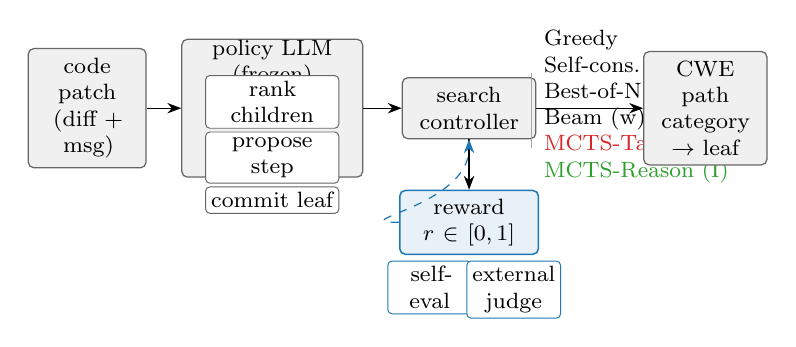
\begin{tikzpicture}[
  execute at begin picture={
    \definecolor{rewardblue}{RGB}{31,119,180}
    \definecolor{mctsred}{RGB}{214,39,40}
    \definecolor{mctsgreen}{RGB}{44,160,44}
  },
  font=\footnotesize,
  >=Stealth,
  box/.style={
    rounded corners=2pt,
    draw=black!60,
    line width=0.45pt,
    align=center,
    inner sep=3.5pt,
    fill=black!6
  },
  smallbox/.style={
    rounded corners=1.5pt,
    draw=black!60,
    line width=0.35pt,
    align=center,
    inner sep=2pt,
    fill=white
  },
  arrow/.style={->, line width=0.45pt},
  reward/.style={
    rounded corners=2pt,
    draw=rewardblue,
    line width=0.55pt,
    align=center,
    inner sep=3pt,
    fill=rewardblue!10
  }
]

\node[box, text width=1.25cm, minimum height=0.78cm] (input) at (0,0)
  {code patch\\(diff + msg)};

\node[box, text width=2.05cm, minimum height=1.75cm] (policy) at (2.35,0)
  {};
\node[align=center] at ([yshift=0.57cm]policy.center) {policy LLM\\(frozen)};
\node[smallbox, text width=1.55cm] (rank) at ([yshift=0.08cm]policy.center)
  {rank children};
\node[smallbox, text width=1.55cm, below=1pt of rank] (prop)
  {propose step};
\node[smallbox, text width=1.55cm, below=1pt of prop] (commit)
  {commit leaf};

\node[box, text width=1.45cm, minimum height=0.76cm] (controller) at (4.85,0)
  {search\\controller};

\node[anchor=west, align=left, inner sep=1pt] (ladder) at (5.76,0.02) {%
  Greedy\\
  Self-cons. (N)\\
  Best-of-N\\
  Beam (w)\\
  {\color{mctsred}MCTS-Tax (I)}\\
  {\color{mctsgreen}MCTS-Reason (I)}%
};
\draw[black!35, line width=0.35pt] ([xshift=-0.12cm,yshift=0.43cm]ladder.west) --
  ([xshift=-0.12cm,yshift=-0.52cm]ladder.west);

\node[reward, text width=1.55cm, minimum height=0.70cm] (reward) at (4.85,-1.45)
  {reward $r\in[0,1]$};
\node[smallbox, draw=rewardblue, text width=0.92cm,
  below left=2pt and -1pt of reward.south] (self) {self-eval};
\node[smallbox, draw=rewardblue, text width=1.05cm,
  below right=2pt and -1pt of reward.south] (judge) {external\\judge};

\node[box, text width=1.32cm, minimum height=0.78cm] (output) at (7.85,0)
  {CWE path\\category $\to$ leaf};

\draw[arrow] (input) -- (policy);
\draw[arrow] (policy) -- (controller);
\draw[arrow] (controller) -- (output);
\draw[arrow] (controller) -- (reward);
\draw[arrow, dashed, draw=rewardblue]
  (reward.west) .. controls +(left:0.75cm) and +(down:0.85cm) .. (controller.south);

\end{tikzpicture}

\caption{Shared architecture. Every strategy drives the same frozen policy LLM
through the same three operations and differs only in the search controller it
plugs in; the reward signal (self-evaluation or external judge) is used only by
the reward-guided strategies (best-of-$N$, beam, MCTS).}
\label{fig:arch}
\end{figure}

\begin{table}[t]
\centering
\small
\begin{tabular}{l l l l}
\toprule
 & Strategy & Searches over & Knob \\
\midrule
M0a & Flat & --- (one call, all leaves) & --- \\
M0b & Greedy & --- (argmax per level) & --- \\
M1 & Self-consistency & i.i.d.\ samples, majority & $N$ \\
M2 & Best-of-$N$ & i.i.d.\ samples, reward-max & $N$ \\
M3 & Beam & taxonomy, width-limited & $w$ \\
M4 & $\mctstax$ & taxonomy, reward-guided & $I$ \\
M5 & $\mctsreas$ & reasoning steps, reward-guided & $I$ \\
\bottomrule
\end{tabular}
\caption{The ladder of strategies, ordered by increasing search structure. All
share one policy, prompt, and output schema; each strategy's knob is set by the
compute-matched protocol (\S\ref{sec:experiments}).}
\label{tab:ladder}
\end{table}

\subsection{No-search baselines}
\textbf{Flat (M0a):} a single call lists all leaf candidates and the model picks
one. \textbf{Greedy-hierarchical (M0b):} one call per level, taking the argmax
child; defines $\Acc_{\text{Greedy}}$ and the policy-strength proxy $\polacc$.

\subsection{Sampling strategies}
\textbf{Self-Consistency (M1):} sample $N$ independent paths at temperature
$T>0$, return the majority leaf. \textbf{Best-of-$N$ (M2):} sample $N$ paths,
return the one maximizing the reward $r$ (\S\ref{sec:reward}). M1 isolates the
value of sampling alone; M2 adds the value of a reward signal.

\subsection{Structured search}
\textbf{Beam (M3):} maintain the top-$w$ partial paths per level under $r$;
deterministic given $\policy$. \textbf{$\mctstax$ (M4):} MCTS over the taxonomy.

\begin{algorithm}[t]
\caption{$\mctstax$: MCTS over the CWE taxonomy}
\label{alg:mcts}
\begin{algorithmic}[1]
\Require code $c$, taxonomy $\mathcal{T}$, policy $\policy$, reward $r$, budget $I$ iterations
\State root state $s_0 \gets (r)$ \Comment{partial path}
\For{$i = 1, \dots, I$}
  \State \textbf{Select}: descend by $Q(s,a) + c_{\text{exp}} \, P(a)\sqrt{N(s)+1}/(1+N(s,a))$ \Comment{PUCT; $P$ from policy scores}
  \State \textbf{Expand}: $\policy$ scores the children of the selected node; scores become priors $P$
  \State \textbf{Evaluate}: $r(s')$ scores the (partial/complete) path via self-eval or judge
  \State \textbf{Backprop}: update $Q,N$ up the search tree
\EndFor
\State \Return path through most-visited children (robust child)
\end{algorithmic}
\end{algorithm}

\textbf{$\mctsreas$ (M5):} the same selection/backup core, but search-tree nodes
are \emph{reasoning states} (a sequence of short free-form reasoning steps about
the patch), not CWE nodes. Each move either appends one reasoning step or
\emph{commits} to a single leaf CWE from the flat leaf list (prompts in
Appendix~\ref{app:prompts}); rollouts force a commit and score the resulting
root-to-leaf path, and the committed leaf is deterministically mapped to a
taxonomy path. Crucially, M5 never commits level-by-level: the coarse category is
implied by the final leaf, not chosen first. M4 vs.\ M5 is our test of whether
search over the output structure or over reasoning is more robust to early-level
compounding (Proposition~\ref{prop:cascade}).

\begin{figure}[t]
\centering
\begin{tikzpicture}[
  execute at begin picture={
    \definecolor{mctsred}{RGB}{214,39,40}
    \definecolor{mctsgreen}{RGB}{44,160,44}
  },
  font=\footnotesize,
  >=Stealth,
  node/.style={inner sep=1pt},
  tax/.style={
    circle,
    draw=black!60,
    line width=0.4pt,
    minimum size=0.34cm,
    inner sep=1pt,
    fill=black!5
  },
  leaf/.style={
    rounded corners=1.5pt,
    draw=black!60,
    line width=0.35pt,
    align=center,
    inner sep=2pt,
    fill=black!4
  },
  step/.style={
    rounded corners=2pt,
    draw=black!60,
    line width=0.4pt,
    align=center,
    inner sep=2.2pt,
    fill=black!5,
    text width=1.42cm
  },
  commit/.style={
    rounded corners=2pt,
    draw=mctsgreen,
    line width=0.45pt,
    align=center,
    inner sep=2.2pt,
    fill=mctsgreen!10,
    text width=1.10cm
  },
  edge/.style={->, line width=0.4pt},
  sel/.style={->, line width=0.85pt, draw=mctsred},
  faint/.style={black!28},
  greenedge/.style={draw=mctsgreen}
]

\node[align=center] at (1.85,1.15) {MCTS-Tax: search over taxonomy};
\node[tax] (root) at (1.85,0.55) {R};
\node[tax] (cat1) at (0.65,-0.15) {A};
\node[tax] (cat2) at (1.85,-0.15) {B};
\node[tax] (cat3) at (3.05,-0.15) {C};
\node[leaf] (a1) at (0.30,-0.90) {leaf};
\node[leaf] (a2) at (1.00,-0.90) {leaf};
\node[leaf, draw=black!28, text=black!38, fill=black!2] (b1) at (1.50,-0.90) {leaf};
\node[leaf, draw=black!28, text=black!38, fill=black!2] (b2) at (2.20,-0.90) {leaf};
\node[leaf] (c1) at (3.05,-0.90) {leaf};

\draw[sel] (root) -- (cat1);
\draw[edge] (root) -- (cat2);
\draw[edge] (root) -- (cat3);
\draw[edge] (cat1) -- (a1);
\draw[edge] (cat1) -- (a2);
\draw[edge, faint] (cat2) -- (b1);
\draw[edge, faint] (cat2) -- (b2);
\draw[edge] (cat3) -- (c1);

\node[align=center, text width=1.85cm, text=mctsred]
  at (1.00,-1.65) {commits at level 0\\unrecoverable};
\draw[mctsgreen, line width=0.55pt]
  ([xshift=-0.13cm,yshift=0.16cm]b2.north east) -- ++(0.08cm,-0.09cm) -- ++(0.17cm,0.20cm);
\node[align=center, text=black!45] at (1.85,-1.20) {unreachable};

\node[align=center] at (6.25,1.15) {MCTS-Reason: search over reasoning};
\node[step] (s0) at (4.65,0.45) {step:\\UAF risk};
\node[step] (s1) at (6.05,0.82) {step:\\realloc moves};
\node[step] (s2) at (6.05,0.06) {step:\\alias stale};
\node[commit] (k1) at (7.45,0.82) {commit:\\CWE-416};
\node[commit] (k2) at (7.45,0.06) {commit:\\CWE-416};
\node[leaf] (l1) at (8.25,0.82) {leaf};
\node[leaf] (l2) at (8.25,0.06) {leaf};

\draw[edge] (s0) -- (s1);
\draw[edge] (s0) -- (s2);
\draw[edge, greenedge] (s1) -- (k1);
\draw[edge, greenedge] (s2) -- (k2);
\draw[edge, greenedge] (k1) -- (l1);
\draw[edge, greenedge] (k2) -- (l2);

\node[align=center, text width=2.25cm, text=mctsgreen]
  at (6.35,-0.95) {defers commitment,\\picks leaf directly};

\end{tikzpicture}

\caption{The two MCTS search spaces. $\mctstax$ (left) walks the label tree and
must pick a coarse category before it has reasoned about the patch; a wrong
first move makes the gold leaf unreachable. $\mctsreas$ (right) searches over
short free-form reasoning steps and commits to a leaf directly, so the category
is implied by the final choice rather than locked in first.}
\label{fig:spaces}
\end{figure}

\subsection{Reward signal}
\label{sec:reward}
We deliberately use \emph{only} zero-shot reward sources, with no trained process
reward model (PRM), to keep the study GPU-free and reproducible:
\begin{itemize}
\item \textbf{Self-eval:} the policy $\policy$ scores its own (partial) path in
$[0,1]$.
\item \textbf{External judge:} a separate, typically stronger model scores the
path given $c$ and candidate CWE descriptions. We record the pair
$(\policy, \text{judge})$.
\end{itemize}
Comparing self-eval vs.\ judge directly probes whether the bottleneck is the
policy or the reward (RQ3/H3). A trained PRM is left to future work
(\S\ref{sec:conclusion}).

\subsection{Structured outputs}
Each policy call returns JSON --- per-candidate scores plus a one-sentence
rationale that is carried into the next level's prompt --- parsed defensively
with a small floor score for missing candidates, so malformed outputs never
crash the search (Appendix~\ref{app:prompts}). Conformal calibration of
path-level prediction sets from the score vectors is part of the final protocol.

\section{Experimental Setup}
\label{sec:experiments}

\paragraph{Research questions and hypotheses.}
\textbf{RQ1} (compute-matched): does MCTS exceed cheaper search at equal token
budget? \textbf{RQ2} (policy): how does the marginal search gain $\gain$ depend on
policy strength $\polacc$? \textbf{RQ3} (reward): is the bottleneck the policy or
the reward? \textbf{RQ4} (search space): taxonomy vs.\ reasoning search?
The corresponding hypotheses are
\textbf{H1} $\Acc_{\mctstax}(\budget) - \Acc_{\text{SC}}(\budget) \le \epsilon$ for
weak policies;
\textbf{H2} $\gain$ increases in $\polacc$ with a threshold $\alpha^\star$ below
which $\gain \le 0$;
\textbf{H3} switching self-eval$\to$judge moves leaf accuracy by $\ll$ the gain
from a stronger policy;
\textbf{H4} reasoning search beats taxonomy search for weak policies.

\subsection{Datasets and Splits}
All examples come from BigVul \citep{fan2020bigvul}: vulnerability-fixing
commits in C/C++ projects rendered as unified diffs with the commit message
(Appendix~\ref{app:data}). The dev set ($n{=}50$, prompt iteration only) is
drawn from BigVul's validation split and the evaluation pool ($n{=}500$,
stratified by CWE) from its test split, so prompt development cannot overfit
the evaluation data. The CWE trees (operational and full-depth,
\S\ref{sec:problem}) are built from MITRE relationships and released with
SHA-256 hashes. A temporal split by CVE year is reported as a robustness check
(\S\ref{sec:analysis}).

\paragraph{Pretraining-leakage control.}
LLMs may have seen public CVEs during pretraining; BigVul's CVEs (2006--2019)
all predate every policy's training cutoff, so a post-cutoff ``fair slice'' is
not constructible from this corpus. We instead verify that conclusions are
stable across CVE years (\S\ref{sec:analysis}) and note that leakage shifts
absolute accuracies, not the within-budget strategy comparisons that are the
object of study --- all strategies share the same policy and examples.

Data statistics (sources, splits, per-category composition, tree hashes) are
given in Appendix~\ref{app:data}.

\subsection{Strategies and Models}
The seven strategies of \S\ref{sec:method} all use the same policy and prompt.
We use five policies spanning the strength axis required for H2: four
cheap-tier (GPT-4.1-nano, Gemini-2.5-Flash-Lite, DeepSeek-V3.1 --- open-weight
--- and Claude-Haiku-4.5) plus a premium policy (Claude-Sonnet-4.6) on a
reduced sample for the strong end. The external judge is a model stronger than
the policy it judges (Claude-Haiku-4.5 judging GPT-4.1-nano); each
$(\policy,\text{judge})$ pair is logged.

\subsection{Compute-Matched Protocol}
We measure $\mathrm{tok}_X(c)$ per knob value (Table~\ref{tab:a2}), giving a
budget grid that spans $1\times$--$10\times$ a single greedy pass, and compare
strategies \emph{only} at comparable measured budgets --- including across
search spaces, where we sweep the $\mctsreas$ iteration knob down until its
budget falls below $\mctstax$'s. We additionally analyze sequential depth and
wall-clock latency (\S\ref{sec:analysis}): self-consistency parallelizes
trivially, MCTS does not --- a practically important asymmetry.

\subsection{Metrics and Statistics}
Primary: leaf accuracy, category (level-0) accuracy, hierarchical-$F_1$ on path
edges \citep{kosmopoulos2015evaluation}, and the accuracy-vs-budget curve
$\Acc_X(\budget)$; secondary: tokens/sample and sequential depth. Stochastic
configurations use $5$ seeds on the weak-policy grid and $3$ on the other
policies (deterministic strategies run once); we report mean $\pm$ std across
seeds, and strategy comparisons at comparable budgets use paired McNemar.

\section{Results}
\label{sec:results}

\subsection{RQ1: Search vs.\ Compute (the headline)}

Table~\ref{tab:matched} reports the compute-matched comparison on a \emph{weak}
policy (GPT-4.1-nano) and a \emph{strong} policy (Claude-Haiku-4.5), on BigVul
examples (diff$+$commit-message input, $7$-category code-aligned tree), comparing
greedy, self-consistency, and $\mctstax$ at a token budget where the latter two
spend roughly equally within each policy (nano $n{=}300$/$5$ seeds, Haiku
$n{=}150$/$3$ seeds; the full pairwise significance matrix is in
Appendix~\ref{app:extra}).

\begin{table}[t]
\centering
\small
\begin{tabular}{l cc cc}
\toprule
 & \multicolumn{2}{c}{nano (weak)} & \multicolumn{2}{c}{Haiku (strong)} \\
\cmidrule(lr){2-3}\cmidrule(lr){4-5}
Strategy & Leaf & Cat.\ & Leaf & Cat.\ \\
\midrule
Greedy (no search)         & $14.7$ & $28.7$ & $24.7$ & $46.7$ \\
Self-Consistency ($N{=}8$) & $16.5$ & $31.5$ & $24.0$ & $46.7$ \\
$\mctstax$ ($I{=}16$)      & $\mathbf{22.9}$ & $\mathbf{39.5}$ & $\mathbf{26.6}$ & $44.4$ \\
\midrule
$\gain$ ($\mctstax$ $-$ greedy) & $+8.2$ & $+10.8$ & $+1.9$ & $-2.3$ \\
\bottomrule
\end{tabular}
\caption{Compute-matched test-time search (accuracy \%), weak vs.\ strong policy
(nano $n{=}300$/$5$ seeds; Haiku $n{=}150$/$3$ seeds, greedy and SC deterministic
or $1$ seed). At equal budget, $\mctstax$ lifts the
weak policy by $+8.2$ (leaf) / $+10.8$ (category) points, but the strong policy by
only $+1.9$ / $-2.3$. Self-consistency helps neither. The marginal search gain
$\gain$ \emph{shrinks} as policy strength grows.}
\label{tab:matched}
\end{table}

\textbf{Finding.} (i) On the weak policy, at matched compute, reward-guided tree
search clearly beats both no-search and sampling-without-reward: $\mctstax$ reaches
$22.9\%$ leaf accuracy versus $16.5\%$ (self-consistency) and $14.7\%$ (greedy);
across-seed std is $\le 1.0$. Both gaps are significant by paired McNemar
($\mctstax$ vs.\ greedy $p{=}8\!\times\!10^{-6}$; vs.\ self-consistency
$p{=}2\!\times\!10^{-3}$, $n{=}300$). Self-consistency---majority vote over
independent samples, ignoring the reward---captures only $+1.8$ points, whereas
MCTS, using the same self-evaluation reward to \emph{steer} the search, captures
$+8.2$. Best-of-$N$ ($N{=}8$), which keeps the reward but drops the tree
(independent samples, return the highest-scoring path), lands in between: $+6.4$
leaf points at a \emph{larger} budget ($15.8$k vs.\ $10.7$k tokens). Reading the
three together: the reward signal alone recovers most of the sampling family's
gap to tree search, and the tree adds the rest while spending less. (ii) On the strong policy the same search yields little ($+1.9$ leaf) to
nothing ($-2.3$ category): the strong policy is already near the signal available
in the input, so reward-guided exploration mostly reconfirms or drifts. Test-time
search here acts as a \emph{compensator for weak policies}, not a universal
improvement.

\subsection{RQ2: Search Gain vs.\ Policy Strength}
Across five policy points the marginal search gain $\gain$ of $\mctstax$ over
greedy (category accuracy) \emph{decreases monotonically} with policy strength
$\polacc$:
%
\begin{center}\small
\begin{tabular}{lccccc}
\toprule
Policy & Gemini-FL & nano & DeepSeek & Haiku & Sonnet \\
$\polacc$ (greedy cat.) & $0.28$ & $0.29$ & $0.37$ & $0.47$ & $0.48$ \\
\midrule
$\gain$ ($\mctstax$, cat.) & $+6.7$ & $+10.8$ & $+2.0$ & $-2.3$ & $+1.7$ \\
$\gain$ ($\mctsreas$, cat.) & $+14.2$ & $+19.4$ & $+8.2$ & $-3.8$ & $+2.5$ \\
\bottomrule
\end{tabular}
\end{center}
%
The taxonomy-search gain falls from $+7$--$11$ points at the weak end
($\polacc \approx 0.28$, two independent policies) to $\approx 0 \pm 3$ at the
strong end (Haiku $-2.3$, Sonnet $+1.7$); the reasoning-search gain starts far
higher ($+14$--$19$) and collapses onto the same near-zero band ($-3.8$ /
$+2.5$). At the strong end the residual gains are within noise of zero at this scale.

This \textbf{contradicts our pre-registered H2}, which anticipated that gain would
\emph{increase} with $\polacc$ (a threshold $\alpha^\star$ below which search
fails). The data show the opposite ordering: search is most valuable exactly where
the policy is weakest, and vanishes as the policy approaches the accuracy ceiling
imposed by the task/labels (\S\ref{sec:analysis}). We therefore revise the claim:
test-time search trades compute for accuracy on under-powered policies, and offers
diminishing-to-negative returns on strong ones.

One nuance: on the mid-strength policy (DeepSeek), plain self-consistency
($N{=}8$: $28.2$ leaf) actually edges out $\mctstax$ ($25.3$) while both trail
$\mctsreas$ ($27.8$ leaf, $44.9$ category) --- so the pre-registered H1
($\mctstax$ within $\epsilon$ of self-consistency at matched budget) fails for
the weak policy but roughly holds mid-scale. The ordering that is stable across
all three policies is the search-space one (RQ4).

\emph{(nano $n{=}300$/$5$ seeds; DeepSeek and Haiku $n{=}130$--$150$/$3$ seeds;
Sonnet $n{=}120$/$1$ seed; all evaluation sets are prefixes of one fixed,
shuffled example file, and greedy is deterministic.)}

\subsection{RQ3: Is the Reward the Bottleneck?}
If reward fidelity limited MCTS, replacing the policy's self-evaluation with a
stronger external judge (Claude-Haiku-4.5, the strong policy of RQ1, judging the
weak nano policy) should help. On matched examples ($n{=}300$, $3$ seeds):
for $\mctstax$ ($I{=}16$) the judge changes nothing --- $22.8 \pm 0.5$ leaf
accuracy vs.\ $22.9 \pm 0.1$ with self-evaluation --- while costing $71\%$ more
tokens ($18.3$k vs.\ $10.7$k). For $\mctsreas$ ($I{=}8$) the judge yields a small
gain ($35.4 \pm 0.6$ vs.\ $33.9 \pm 0.3$) at $27\%$ more tokens; but self-eval
$\mctsreas$ at $I{=}2$ already reaches $34.8 \pm 0.4$ at less than a \emph{third}
of the judge configuration's budget, so the gain does not survive compute
matching.

\textbf{Finding.} Upgrading reward fidelity does not move taxonomy search at all
--- its early-commitment pathology is structural, and no reward source can fix a
search-space problem --- and buys, on reasoning search, less than its extra
tokens are worth elsewhere. The reward source is therefore not the binding
constraint; the policy and the search space are (consistent with RQ2 and RQ4).
A reward-calibration analysis (AUROC of rollout reward vs.\ correctness for
both reward sources) corroborates this reading in \S\ref{sec:analysis}.

\subsection{RQ4: Taxonomy vs.\ Reasoning Search}
We compare MCTS over the taxonomy ($\mctstax$, committing level-by-level) against
MCTS over a free-form reasoning trajectory ($\mctsreas$, which reasons and then
commits directly to a leaf), at a comparable budget on the weak policy
(Table~\ref{tab:m4m5}, $n{=}150$).

\begin{table}[t]
\centering
\small
\begin{tabular}{l cc cc}
\toprule
 & \multicolumn{2}{c}{nano (weak)} & \multicolumn{2}{c}{Haiku (strong)} \\
\cmidrule(lr){2-3}\cmidrule(lr){4-5}
Strategy & Leaf & Cat.\ & Leaf & Cat.\ \\
\midrule
Greedy                & $14.7$ & $28.7$ & $24.7$ & $46.7$ \\
$\mctstax$ ($I{=}16$) & $22.9$ & $39.5$ & $26.6$ & $44.4$ \\
$\mctsreas$ ($I{=}8$) & $\mathbf{33.9}$ & $\mathbf{48.1}$ & $\mathbf{28.4}$ & $42.9$ \\
\bottomrule
\end{tabular}
\caption{Taxonomy vs.\ reasoning search (accuracy \%; nano $n{=}300$/$5$ seeds,
Haiku $n{=}150$/$3$ seeds). Reasoning search beats taxonomy search on \emph{both}
policies; the margin is large for the weak policy ($+11$ leaf) and modest for the
strong one ($+1.8$).}
\label{tab:m4m5}
\end{table}

\textbf{Finding.} Reasoning-trajectory search dominates taxonomy search on
\emph{both} policies (weak: $33.9$ vs.\ $22.9$ leaf, $+11$, paired McNemar
$p{=}3.2\!\times\!10^{-4}$, $n{=}300$; strong: $28.4$ vs.\ $26.6$, $+1.8$), with
the advantage shrinking as the policy strengthens (cf.\ RQ2). On the strong
policy it trades a small category drop ($42.9$ vs.\ greedy $46.7$) for a leaf
gain, reaching finer leaves at the cost of occasionally landing in a neighbouring
category. On the premium policy (Sonnet, $n{=}120$, $1$ seed) the ordering
\emph{reverses} on leaf accuracy ($31.7$ vs.\ $35.0$ for $\mctstax$): a policy
that already reasons well in a single pass gains nothing from an external
reasoning scaffold, while the taxonomy structure still adds a little fine-grained
discrimination. The search-space advantage, like the search gain itself, is a
property of \emph{weak-to-mid} policies.

\paragraph{Strict budget matching.}
Sweeping $\mctsreas$ over $I \in \{2,4,6,8\}$ ($n{=}300$, $5$ seeds,
Figure~\ref{fig:budget}) shows its accuracy is \emph{flat in the iteration count}:
$I{=}2$, at $5.3$k tokens/example --- \emph{half} of $\mctstax$'s $10.7$k budget
--- already reaches $34.8\%$ leaf / $50.4\%$ category accuracy, slightly
\emph{above} $I{=}8$ ($33.9$ / $48.1$). The dominance over taxonomy search
therefore survives strict budget matching with room to spare ($\mctsreas$ at
$I{=}2$ vs.\ $\mctstax$ at $I{=}16$: paired McNemar $p{=}8.7\!\times\!10^{-5}$;
vs.\ greedy: $p{=}4.4\!\times\!10^{-10}$). The flatness is itself informative:
nearly all of $\mctsreas$'s gain comes from its \emph{representation} --- reason
first, commit to a leaf directly --- rather than from accumulating search
statistics; we return to this in \S\ref{sec:analysis}.

The mechanism is the cascade (Proposition~\ref{prop:cascade}): $\mctstax$ commits
to a category at level~0 and cannot recover the correct leaf once that choice is
wrong, whereas $\mctsreas$ defers commitment, reasons over the patch, and selects
a leaf directly---side-stepping early-level lock-in. The error breakdown ($5$
seeds $\times$ $300$ examples, Figure~\ref{fig:cascade}) confirms this:
$\mctstax$ commits to a wrong category on $60.5\%$ of examples (unrecoverable by
construction) versus $51.9\%$ for $\mctsreas$, and on the cases where $\mctstax$
picks the wrong category, $\mctsreas$ recovers the correct one $25.7\%$ of the
time. Strikingly, the weak policy with reasoning search reaches category accuracy
($50.4\%$ at $I{=}2$) \emph{above} the strong policy's greedy accuracy ($46.7\%$,
Table~\ref{tab:matched}).

\begin{figure}[t]
\centering
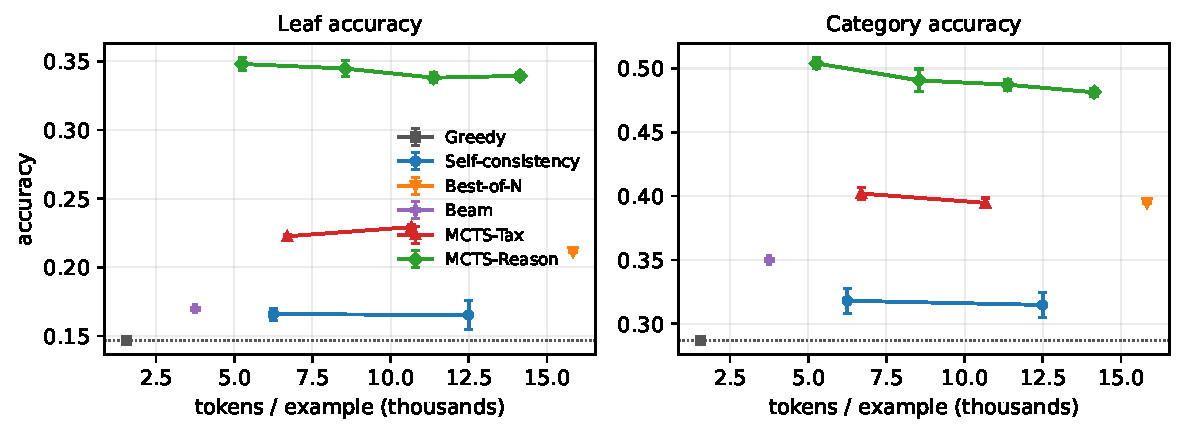
\includegraphics[width=\linewidth]{figures/budget_curve.pdf}
\caption{Accuracy vs.\ token budget (GPT-4.1-nano, $n{=}300$, mean $\pm$ std over
$5$ seeds; greedy, beam, and best-of-$N$ are single runs). $\mctsreas$ dominates
at every budget and is flat in its iteration knob; $\mctstax$ saturates between
$I{=}8$ and $I{=}16$; best-of-$N$ (reward, no tree) sits between
self-consistency and $\mctstax$; self-consistency barely improves on greedy.
What is searched matters far more than how much.}
\label{fig:budget}
\end{figure}

\section{Analysis}
\label{sec:analysis}

\subsection{When does search pay off?}
Synthesizing RQ1--RQ4 yields a simple decision rule for test-time search on this
structured-output task:
\begin{enumerate}
\item \textbf{Search the reasoning, not the taxonomy --- for weak-to-mid
policies.} $\mctsreas$ beats $\mctstax$ on four of five policies
(Table~\ref{tab:m4m5}), and on the weak policy even at \emph{half} the budget
(Figure~\ref{fig:budget}); committing to coarse categories early is the single
most costly design choice. On the premium policy the two are within noise of
each other and of greedy.
\item \textbf{Spend on search when the policy is weak.} The marginal gain over
greedy is large for a weak policy and shrinks toward zero as policy strength
$\polacc$ grows (RQ2); on a strong policy near the task's accuracy ceiling,
additional search is barely worth its cost.
\item \textbf{Prefer reward-guided search to sampling.} At matched budget,
self-consistency---which ignores the reward---captures almost none of the gain that
reward-guided MCTS does (RQ1).
\end{enumerate}
The binding constraints are the \emph{search space} and the \emph{policy}, not the
search budget or the reward source.

\subsection{Cascade error: why taxonomy search hurts}
Proposition~\ref{prop:cascade} predicts that level-by-level commitment compounds
early mistakes. The per-example breakdown (weak policy, $5$ seeds $\times$
$n{=}300$, Figure~\ref{fig:cascade}) confirms it: \textbf{$\mctstax$ commits to a
wrong category --- unrecoverable by construction --- on $60.5\%$ of examples,
versus $51.9\%$ for $\mctsreas$} (greedy: $71.3\%$), and on the examples where
$\mctstax$ chose the wrong category, $\mctsreas$ recovered the correct one
$25.7\%$ of the time. Notably, the within-category error rate (right category,
wrong leaf) is nearly constant across strategies ($14$--$17\%$): all of the
reasoning-search advantage comes from avoiding the early, coarse commitment, not
from finer leaf discrimination. Deferring commitment is thus the mechanism behind
reasoning search's advantage.

\begin{figure}[t]
\centering
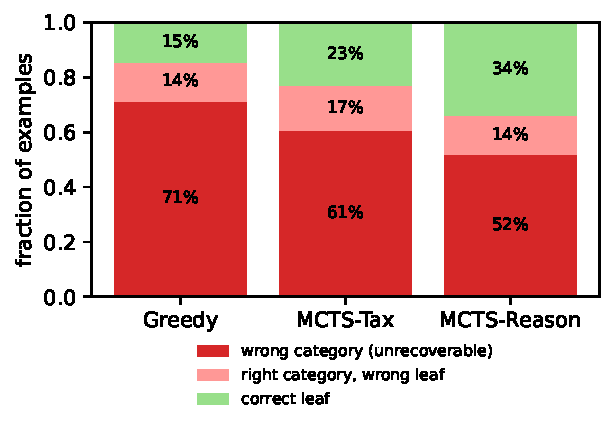
\includegraphics[width=0.8\linewidth]{figures/cascade.pdf}
\caption{First-error level (GPT-4.1-nano, $5$ seeds $\times$ $300$ examples;
greedy is deterministic, $1$ seed). Strategies differ almost entirely in how
often they commit to a wrong coarse category; the right-category-wrong-leaf band
is nearly constant.}
\label{fig:cascade}
\end{figure}

\subsection{The scaffold, not the search}
The $\mctsreas$ budget sweep (Figure~\ref{fig:budget}) adds a sharper reading of
RQ4: accuracy at $I{=}2$ --- where the ``tree'' has barely expanded beyond its
root and the reward has had no opportunity to steer --- already matches $I{=}8$.
Most of the benefit of ``MCTS over reasoning'' is therefore attributable to its
\emph{scaffold} (generate free-form reasoning about the patch, then commit to a
leaf directly, skipping level-by-level commitment), not to the tree-search
machinery on top. This refines the headline: the search-space design dominates
both the budget \emph{and the amount of search itself}. By contrast, $\mctstax$
does benefit from iterations at small $I$ (Figure~\ref{fig:budget}), but
saturates by $I{\approx}8$ at a level far below the reasoning scaffold. The
scaffold reading also explains the premium-policy reversal (RQ4): externalized
step-by-step reasoning is a crutch the strongest policy no longer needs, so what
remains useful there is only the taxonomy's fine-grained discrimination.

\subsection{Reward fidelity is not the bottleneck}
Replacing self-evaluation with a stronger external judge (Claude-Haiku-4.5
judging GPT-4.1-nano) leaves taxonomy search exactly where it was ($22.8$ vs.\
$22.9$ leaf) and lifts reasoning search by $+1.5$ points at $+27\%$ tokens ---
less than the same tokens buy via the search-space choice itself (RQ3). The
asymmetry is informative: in $\mctstax$ the reward only re-ranks siblings
\emph{after} the category commitment that drives most errors
(Figure~\ref{fig:cascade}), so no reward source can rescue it; in $\mctsreas$
the reward selects among complete leaf commitments, where a better judge has
something to act on --- yet the effect is marginal because the policy's own
self-evaluation already separates its candidate commitments about as well.

The logged rollout rewards quantify this directly. Treating the reward of each
MCTS rollout as a predictor of whether that rollout's leaf is correct: on
taxonomy rollouts the judge is \emph{measurably better calibrated} than
self-evaluation (AUROC $0.76$ vs.\ $0.71$, $14$--$24$k pooled rollouts) --- and
final accuracy still does not move, confirming that reward quality is not what
limits $\mctstax$. On reasoning rollouts the judge is \emph{no} better
calibrated ($0.62$ vs.\ $0.64$), consistent with its marginal accuracy effect
there. In both cases the reward ranks candidates far above chance, so the
search is reward-guided in a meaningful sense; it is the set of candidates the
search space exposes, not their ranking, that binds.

\subsection{Latency and practical cost}
Token budget understates MCTS's practical cost, and the right structural
measure is \emph{sequential depth}: the number of LLM rounds that cannot be
parallelized. On our two-level tree, greedy and self-consistency have depth $2$
(samples are independent), best-of-$N$ depth $3$, and beam depth equal to the
number of levels; MCTS iterations, by contrast, are inherently sequential
because each depends on the previous tree statistics --- roughly $2I$ rounds
for $\mctstax$ ($\approx\!34$ at $I{=}16$) and $3I$ for $\mctsreas$
($\approx\!24$ at $I{=}8$, $\approx\!7$ at $I{=}2$). Uncached pilot runs are
consistent: with 10-way example parallelism, Haiku spends $\approx\!47$\,s and
$\approx\!32$\,s of wall clock per example on $\mctstax(16)$ and
$\mctsreas(8)$ respectively, versus seconds for the depth-2 strategies. The
flat $\mctsreas$ iteration curve (Figure~\ref{fig:budget}) is therefore also a
latency result: at $I{=}2$ the best strategy runs at near-interactive depth,
whereas matching $\mctstax$'s budget costs an order of magnitude more
sequential rounds for less accuracy.

\subsection{Failure modes}
We decompose the errors of $\mctstax(16)$ and $\mctsreas(8)$ (weak policy, seed
13, $n{=}300$) along three mechanically computable axes plus one adjudicated
one. \emph{Level:} both strategies make $78\%$ of their errors at the category
level and $22\%$ at the sibling level --- the strategies differ in \emph{how
many} errors they make (231 vs.\ 198), not where. \emph{Reward misranking:} the
gold leaf appeared among the search's own rollout commitments --- found but not
selected --- in $17\%$ of $\mctstax$ errors and $27\%$ of $\mctsreas$ errors;
this slice is the upper bound on what a better reward could recover, and its
size for $\mctsreas$ explains why the external judge helps only there (RQ3).
\emph{Ambiguous gold:} an LLM adjudicator (Claude-Haiku-4.5, shown the patch
and both labels' definitions) judges the model's label a \emph{defensible
alternative} for $42\%$ of sampled $\mctsreas$ errors but only $12\%$ of
$\mctstax$ errors ($50$ samples each). Reasoning search's residual errors are
thus to a large degree single-label artifacts on genuinely multi-label
examples, whereas taxonomy search's errors are mostly outright misses ---
its effective accuracy gap is wider than the headline numbers suggest.

\subsection{Limitations}
\label{sec:limitations}
\begin{itemize}
\item \textbf{Label noise and ambiguity.} BigVul CWE labels are known to be noisy,
and many functions admit several valid CWEs while the gold label is single; this
caps achievable accuracy independently of method (greedy category accuracy plateaus
near $0.40$ even for a premium model on raw functions).
\item \textbf{Scale.} Comparisons use $n{=}300$ ($5$ seeds) for the weak policy
and $n{=}120$--$150$ ($1$--$3$ seeds) for the others, all drawn from one fixed
example file (the smaller sets are prefixes of the larger), with a few per-cell
API failures dropped. The headline effects are large relative to this scale
(across-seed std $\le 1.1$ points; Bonferroni-corrected significance in
Appendix~\ref{app:extra}), but the premium-policy cells in particular would
benefit from more data.
\item \textbf{Saturation of $\mctstax$.} We compare $\mctstax$ up to $I{=}16$
($10.7$k tokens); deeper probes ($I$ up to $128$, full-depth tree, $n{=}8$)
showed predictions frozen well before $I{=}16$, and $\mctsreas$ at \emph{half}
$\mctstax$'s budget already dominates
(Figure~\ref{fig:budget}), so larger taxonomy-search budgets are unlikely to
change the conclusion.
\item \textbf{Reward is zero-shot only.} A trained process reward model could shift
the RQ3 conclusion; we leave it to future work.
\item \textbf{Pretraining exposure.} We cannot fully rule out that LLMs saw test
CVEs during pretraining; a post-cutoff slice is a planned robustness check.
\item \textbf{Granularity coverage.} Findings are established on a 26-CWE
subset of View-1003 (the labels occurring in the data) plus a floor probe at
View-1000; the intermediate regime --- the full 130-CWE View-1003 as used by
NVD --- is the natural target for future work.
\item \textbf{Language coverage.} Data is C/C++-dominated.
\end{itemize}

\subsection{Tree granularity as a boundary condition}
\label{sec:granularity}
Does the picture survive at the full Research-Concepts granularity (View-1000,
$716$ leaves)? A probe ($n{=}50$) says the question itself dissolves there: the
\emph{strongest} policies drop to near-floor --- Sonnet greedy reaches $20\%$
pillar accuracy (10 pillars) and its predicted path passes through the gold node
on only $6\%$ of examples; $\mctstax$ ($I{=}16$), now spending $30$k
tokens/example, lifts this to $28\%$ / $14\%$. Search still moves the needle
(gold-on-path doubles), but from a base so low that no test-time budget makes
the output usable. This is the boundary condition our policy-strength story
predicts: search converts headroom into accuracy only when the policy is above
the floor of the label space (RQ2), and at research granularity it is not ---
which is also why MITRE directs practical CVE mapping to the smaller View-1003
(\S\ref{sec:problem}). Test-time search is a lever \emph{within} the
operational regime, not a way to buy back a label space the policy cannot see.

\subsection{Temporal robustness}
Splitting the $300$ pilot examples by CVE year (2006--16: $n{=}168$; 2017--19:
$n{=}132$) preserves the full strategy ordering in both periods
(weak policy, leaf accuracy, $5$ seeds): greedy $11.3$/$18.9$,
self-consistency $12.4$/$21.8$, $\mctstax$ $16.0$/$31.8$, $\mctsreas$
$33.2$/$35.6$ (old/recent). All strategies score higher on recent CVEs --- a
drift we cannot attribute (different project mix, or greater pretraining
exposure to recent CVEs) --- but the conclusions rest on \emph{within-period}
orderings, which are stable; notably $\mctsreas$ is the least sensitive to the
period ($+2.4$ points old$\to$recent vs.\ $+15.8$ for $\mctstax$).
\section{Conclusion}
\label{sec:conclusion}

We presented a compute-matched study of test-time search for hierarchical CWE
classification, holding the policy LLM and prompt fixed and comparing seven
strategies at equal token budgets. By isolating policy strength and reward
fidelity, we separate the value of \emph{search structure} from the value of
\emph{extra compute} --- a confound that pervades reported MCTS-for-LLM gains.

Searching a free-form reasoning trajectory beats searching the output taxonomy by
$+12$ leaf points at \emph{half} the token budget on the weak policy
($p{<}10^{-4}$), and on four of five policies overall, because taxonomy search
commits to coarse categories early and compounds the error---making the
\emph{search space} the primary design lever, above budget or reward. The margin
closes, and at the premium end reverses, as the policy strengthens: a policy that
reasons well unaided no longer needs the scaffold. Indeed, the reasoning
strategy's accuracy is flat in its iteration knob: the scaffold (reason, then
commit to a leaf directly), not the tree search on top, carries the gain. At matched compute, reward-guided tree search also delivers a clear gain on
a weak policy ($+8.2$ leaf points over greedy, $+6.4$ over self-consistency) but a
negligible one on a strong policy ($+1.9$); self-consistency---sampling without a
reward---helps neither. The marginal value of search thus \emph{decreases} with
policy strength, contradicting the intuition that better policies search better.
The binding constraint is the accuracy ceiling of the policy on the task, not the
search budget: once a policy nears that ceiling, additional search reconfirms or
drifts. We read this as a budget-aware rule (\S\ref{sec:analysis}): spend on search
when the policy is weak and the reward is informative; spend on a better policy
otherwise.

\paragraph{A budget-aware decision rule.}
Our main practical deliverable is a rule for \emph{when} to spend on search:
read off the policy's pillar accuracy $\polacc$ and the available budget
$\budget$, then choose greedy, self-consistency, or MCTS accordingly
(\S\ref{sec:analysis}).

\paragraph{Future work.}
A trained process reward model (PRM) could shift the reward-bottleneck
conclusion; we left it out to keep the study GPU-free, and flag it as the most
informative next experiment. Extending the protocol to multi-language data and to
detection/localization (beyond classification) are natural follow-ups.

\paragraph{Broader Impact.}
LLM-assisted vulnerability triage is already deployed under tight cost budgets;
our results give practitioners a calibrated answer to ``is structured search
worth its tokens here?''---often the answer is to fix the input representation
and the search space before buying more compute, which lowers both cost and the
energy footprint of security tooling. At the same time, automated CWE labels are
a triage aid, not a verdict: our best configuration still mislabels most
samples at the leaf level, and a false negative can hide a real weakness.
Deployments should keep a human reviewer in the loop and treat predicted labels
as prioritization signals rather than ground truth. The study uses only public,
already-disclosed vulnerabilities and fixes, so it does not create new
disclosure risk.


\bibliographystyle{plainnat}
\bibliography{references}

\appendix
\section{Dataset Construction Details}
\label{app:data}

This appendix documents the data actually used in the pilot experiments
(\S\ref{sec:results}); steps that belong to the final protocol but are not yet
exercised by the pilot are explicitly marked \emph{planned}.

\subsection{Source and input construction (pilot)}
All pilot examples come from BigVul \citep{fan2020bigvul}, which provides, for
each vulnerability-fixing commit in C/C++ projects, the vulnerable function
(\texttt{func\_before}), the fixed function (\texttt{func\_after}), the commit
message, and a CVE-derived CWE label. We keep rows marked vulnerable whose CWE
normalizes to a leaf of our tree (below), and render each example as a
\emph{unified diff} from the vulnerable to the fixed function, prefixed by an
instruction comment (``\texttt{'-'} lines are the VULNERABLE code \ldots
classify the weakness in the removed/vulnerable code'') and the first 500
characters of the commit message. The diff localizes the vulnerable lines and is
the input representation under which models clear the $\approx\!40\%$ category
ceiling we observed on raw functions. Diffs with fewer than three lines are
dropped; code is truncated at 5{,}000 characters at prompt time
(\S\ref{app:prompts}).

\subsection{Splits (pilot)}
The dev set ($n{=}50$) is drawn from the BigVul validation split and the pilot
set ($n{=}500$) from the BigVul test split --- so prompt iteration on dev cannot
overfit the pilot --- using per-CWE stratified round-robin sampling (seed 42).
Pilot statistics: 500 examples, 18 distinct CWE leaves, 73 distinct projects;
median diff length 15 lines (mean 27). Category composition:
\textsc{buffer} 214, \textsc{injection} 117, \textsc{access} 77,
\textsc{lifetime} 54, \textsc{numeric} 28, \textsc{resource} 5,
\textsc{control} 5; the largest leaves are CWE-119 (128), CWE-20 (112),
CWE-125 (68), CWE-200 (49). Most reported runs use the first 300 (nano) or 150
(Haiku, DeepSeek) examples of this fixed, shuffled file; per-example outputs are
released for paired analyses.

\subsection{CWE trees}
\paragraph{Full tree.} We download the official MITRE CWE corpus
(\texttt{cwec\_latest.xml}), extract the Research-Concepts view (View-1000)
ChildOf hierarchy rooted at the ten Pillars, and resolve multi-parent nodes to a
\emph{primary} parent by breadth-first search from the pillars (first, i.e.\
minimal-depth, discovery wins). The result has 944 nodes and 716 leaves (depths
0--5) and is released as adjacency JSON with SHA-256
\texttt{7aeff209\ldots{}26948a6}.

\paragraph{Coarse code-aligned tree (pilot).} MITRE pillars are research
abstractions (``Improper Control of a Resource Through its Lifetime'') that even
strong policies place poorly, which floors level-0 accuracy and makes the
policy-strength axis (RQ2) unreadable. For the pilot we therefore regroup the
22 dataset CWEs into a 2-level tree with 7 code-recognizable super-categories
(spatial memory, temporal memory / lifetime, resource exhaustion, numeric,
injection / input handling, control-flow, access control / info exposure /
misc); leaves keep their MITRE names and descriptions. All $26$ leaves are
members of CWE View-1003, the simplified-mapping view that NVD uses to label
published CVEs, so this label space is a subset of the official operational
vocabulary rather than an ad-hoc simplification. The tree is released with
SHA-256 \texttt{f3013c19\ldots{}9c79aa}. The full-depth tree is used only for
the granularity boundary-condition probe (\S\ref{sec:granularity}).

\subsection{Multi-source pooling and deduplication (planned)}
The final protocol pools PrimeVul \citep{ding2024primevul}, DiverseVul
\citep{chen2023diversevul}, BigVul, and CVEfixes \citep{bhandari2021cvefixes},
with function-level MinHash deduplication (Jaccard $\ge 0.85$) and
repository-level disjointness across splits; the pilot uses a single source
(BigVul) with splits inherited from the dataset's own validation/test
partition, so cross-source leakage is not yet a concern at pilot scale.

\subsection{Pretraining-leakage slice (planned)}
Because public CVEs may appear in pretraining corpora, the final protocol
reports a slice restricted to CVEs published after each model's training
cutoff. At pilot scale we note that all four policies see the same examples, so
leakage would shift absolute numbers rather than the strategy comparisons that
are the object of study.

\subsection{Datasheet (planned)}
A Datasheets-for-Datasets \citep{gebru2021datasheets} entry (motivation,
composition, collection, preprocessing, uses, distribution, maintenance) will
accompany the released benchmark bundle.

\section{Prompts and Schemas}
\label{app:prompts}

All strategies share a single per-step policy prompt (\S\ref{app:rank}); the
reasoning-trajectory strategies add two prompts of their own
(\S\ref{app:reason}); both reward sources share one scoring prompt
(\S\ref{app:reward}). All calls request \texttt{response\_format
= json\_object} and are parsed defensively: malformed entries are dropped, and
any candidate missing from the output receives a floor score of $10^{-3}$ so
search never crashes on a parse failure. Code longer than 5{,}000 characters is
truncated with an explicit \texttt{/* \ldots truncated \ldots */} marker.

\subsection{Per-step ranking prompt (all taxonomy strategies)}
\label{app:rank}

Greedy, self-consistency, best-of-$N$, beam, and $\mctstax$ all call one shared
step: rank the candidate children of the current taxonomy node. Placeholders are
in angle brackets.

\begin{lstlisting}
SYSTEM:
You are a security expert classifying the vulnerability in a code
function according to the CWE taxonomy. Classify the WEAKNESS the
code exhibits, not the fix. You are given the candidate CWE
categories at one level of the taxonomy; choose among THESE
candidates only.

USER:
[Prior reasoning: <rationale carried over from the parent step>]

Function:
```c
<code, truncated at 5000 chars>
```

Candidate CWE categories:
<one line per child: "- CWE-XXX: <name>. <description>">

Score EVERY candidate listed above by how likely it describes the
weakness in the function (0.0 = no, 1.0 = yes); scores need not
sum to 1. You MUST output an entry for every candidate CWE id.
Return JSON: {"scores": {"CWE-XXX": 0.0, "CWE-YYY": 0.0, ...},
"rationale": "one sentence"}.
\end{lstlisting}

Greedy takes the arg-max at temperature $0$; self-consistency and best-of-$N$
sample the same prompt at temperature $0.7$ with a per-sample cache nonce;
beam and $\mctstax$ use the full score vector as child priors. The
\texttt{rationale} is capped at 300 characters and passed down as ``prior
reasoning'' to the next level.

\subsection{Reasoning-trajectory prompts ($\mctsreas$)}
\label{app:reason}

$\mctsreas$ searches over reasoning states rather than taxonomy nodes. A move is
either a brief next reasoning step or a commit to one leaf CWE; the candidate
list shown to the model is the flat list of tree leaves (id $+$ name).

\begin{lstlisting}
SYSTEM:
You are a security expert reasoning step by step about the weakness
in a code patch, in order to classify it into exactly one CWE.
Reason about the removed (vulnerable) lines, not the fix.

USER (expansion; k = 3):
Code patch:
```c
<code, truncated at 5000 chars>
```

Reasoning so far:
<numbered steps, or "(none yet)">

Candidate CWEs:
<one line per leaf: "- CWE-XXX: <name>">

Propose 3 DISTINCT next moves toward the answer. Each move is
either a brief next reasoning step, or a final commit to ONE
candidate CWE id. Return JSON: {"moves": [{"type": "step",
"text": "..."} or {"type": "commit", "cwe": "CWE-XXX"}, ...]}.

USER (forced commit; rollouts and final extraction):
<same code + reasoning-so-far + candidate blocks>

Commit to the single best CWE now. Return JSON {"cwe": "CWE-XXX"}.
\end{lstlisting}

Reasoning steps are capped at 300 characters and traces at
\texttt{max\_steps} $= 3$; a commit to an id outside the candidate list falls
back to the first leaf (and is counted as an error in practice). Expansion runs
at temperature $0$; rollout commits run at temperature $0.7$ with a
\texttt{(seed, iteration)} cache nonce.

\subsection{Reward prompt (self-evaluation and external judge)}
\label{app:reward}

Both reward sources use the \emph{same} prompt; the only difference is the model
it is sent to --- the policy itself (\texttt{self\_eval}) or the stronger judge
(\texttt{external\_judge}, Claude-Haiku-4.5). The reward scores a partial or
complete root-to-node path in $[0,1]$; both are zero-shot, no PRM is trained.

\begin{lstlisting}
SYSTEM:
You are auditing a proposed CWE classification of a code function.
Judge how well the proposed CWE path describes the weakness in the
code. Classify the weakness, not the fix.

USER:
Function:
```c
<code, truncated at 5000 chars>
```

Proposed CWE path: CWE-AAA (<name>) -> CWE-BBB (<name>) -> ...
This path is {PARTIAL (not yet a leaf) | COMPLETE (leaf)}.

Description of the final node CWE-BBB: <description or "n/a">

Return JSON {"score": 0.0-1.0} where score is the probability this
path correctly classifies the weakness in the function.
\end{lstlisting}

The score is clamped to $[0,1]$; a parse failure scores $0$.

\section{Additional Results}
\label{app:extra}

\subsection{Full pilot budget grid (weak policy)}
Table~\ref{tab:a2} reports every (strategy, knob) point behind
Figure~\ref{fig:budget}: GPT-4.1-nano, $n{=}300$, mean $\pm$ std over $5$ seeds
(greedy is deterministic and run once).

\begin{table}[h]
\centering
\small
\begin{tabular}{l r r cc}
\toprule
Strategy & Knob & Tokens/ex & Leaf (\%) & Category (\%) \\
\midrule
Greedy           & ---      & $1{,}561$  & $14.7$            & $28.7$ \\
Self-consistency & $N{=}4$  & $6{,}246$  & $16.6 \pm 0.4$    & $31.8 \pm 1.0$ \\
Self-consistency & $N{=}8$  & $12{,}493$ & $16.5 \pm 1.1$    & $31.5 \pm 1.0$ \\
Best-of-$N$      & $N{=}8$  & $15{,}836$ & $21.1$            & $39.5$ \\
Beam             & $w{=}4$  & $3{,}753$  & $17.0$            & $35.0$ \\
$\mctstax$       & $I{=}8$  & $6{,}695$  & $22.3 \pm 0.1$    & $40.2 \pm 0.4$ \\
$\mctstax$       & $I{=}16$ & $10{,}669$ & $22.9 \pm 0.1$    & $39.5 \pm 0.4$ \\
$\mctsreas$      & $I{=}2$  & $5{,}257$  & $\mathbf{34.8 \pm 0.4}$ & $\mathbf{50.4 \pm 0.4}$ \\
$\mctsreas$      & $I{=}4$  & $8{,}546$  & $34.5 \pm 0.6$    & $49.1 \pm 0.9$ \\
$\mctsreas$      & $I{=}6$  & $11{,}379$ & $33.8 \pm 0.4$    & $48.7 \pm 0.4$ \\
$\mctsreas$      & $I{=}8$  & $14{,}142$ & $33.9 \pm 0.3$    & $48.1 \pm 0.3$ \\
\bottomrule
\end{tabular}
\caption{Pilot budget grid (GPT-4.1-nano, BigVul diff$+$msg, $n{=}300$, $5$
seeds; best-of-$N$ and beam: $1$ seed, best-of-$N$ $n{=}289$ after API
failures). Tokens/ex doubles as the knob$\to$tokens calibration used to set
compute-matched comparison points.}
\label{tab:a2}
\end{table}

Across-seed variance is small throughout (std $\le 1.1$ points), so the pilot's
seed budget is adequate for the gaps being measured.

\subsection{Pairwise significance (weak policy)}
Table~\ref{tab:mcnemar} gives the full strategy $\times$ strategy paired
McNemar matrix on leaf accuracy (seed 13, $n{=}289$--$300$ common examples per
pair). After Bonferroni correction over all $28$ pairs, the picture is sharp:
both $\mctsreas$ variants beat every other strategy; both $\mctstax$ variants
beat greedy and beam; best-of-$N$ is statistically indistinguishable from
$\mctstax$; and the iteration knob does not matter within either MCTS family
($\mctsreas$ $I{=}2$ vs.\ $I{=}8$: $p{=}0.73$; $\mctstax$ $I{=}8$ vs.\ $I{=}16$:
$p{=}0.69$).

\begin{table}[h]
\centering
\scriptsize
\setlength{\tabcolsep}{3.5pt}
\begin{tabular}{l ccccccc}
\toprule
 & SC-8 & BoN-8 & Beam-4 & Tax-8 & Tax-16 & Reas-2 & Reas-8 \\
\midrule
Greedy  & .24 & .013 & .14 & $\mathbf{6\!\cdot\!10^{-6}}$ & $\mathbf{2\!\cdot\!10^{-6}}$ & $\mathbf{4\!\cdot\!10^{-10}}$ & $\mathbf{3\!\cdot\!10^{-9}}$ \\
SC-8    &     & .060 & 1.0 & .005 & .002 & $\mathbf{2\!\cdot\!10^{-8}}$ & $\mathbf{7\!\cdot\!10^{-8}}$ \\
BoN-8   &     &      & .10 & .66  & .55  & $\mathbf{8\!\cdot\!10^{-5}}$ & $\mathbf{1\!\cdot\!10^{-4}}$ \\
Beam-4  &     &      &     & $\mathbf{9\!\cdot\!10^{-4}}$ & $\mathbf{3\!\cdot\!10^{-4}}$ & $\mathbf{5\!\cdot\!10^{-9}}$ & $\mathbf{5\!\cdot\!10^{-8}}$ \\
Tax-8   &     &      &     &      & .69  & $\mathbf{5\!\cdot\!10^{-5}}$ & $\mathbf{2\!\cdot\!10^{-4}}$ \\
Tax-16  &     &      &     &      &      & $\mathbf{9\!\cdot\!10^{-5}}$ & $\mathbf{3\!\cdot\!10^{-4}}$ \\
Reas-2  &     &      &     &      &      &      & .73 \\
\bottomrule
\end{tabular}
\caption{Paired McNemar $p$-values, leaf accuracy, GPT-4.1-nano, seed 13.
Bold: significant after Bonferroni correction over $28$ pairs
($\alpha{=}0.05$).}
\label{tab:mcnemar}
\end{table}

\subsection{Taxonomy-search saturation probe}
On the full-depth MITRE tree (716 leaves), $\mctstax$ at $I \in \{16, 64, 128\}$
returned byte-identical predictions on a small dev probe ($n{=}8$; $13$k, $38$k,
and $71$k tokens/example respectively): once the level-wise priors lock in, more
iterations re-visit the same branch. This motivated capping $\mctstax$ at
$I{=}16$ in the pilot grid.

\subsection{Ablations left to future work}
Pre-registered ablations we did not run: exploration-constant sensitivity
($c_{\text{exp}} \in \{0.5, 1.0, 1.41\}$) and the aggregation rule (majority
vs.\ reward-weighted vs.\ robust-child). Both concern second-order design
choices of the search machinery, which the main results show is not the
binding factor (\S\ref{sec:analysis}); granularity and latency are covered in
\S\ref{sec:granularity} and the latency analysis respectively.


\end{document}
